\chapter{实例章节}
\label{cha:introduction}

以下是简单的示例代码。
\par \textbf{加粗}[title=代码段题目]

\begin{lstlisting}
EFI_STATUS InfoRead(char *FileName,char *Buf)
{
    EFI_STATUS Status=0; //4个空格
    EFI_FILE_PROTOCOL *FileHandle=0; //4个空格
	EFI_FILE_PROTOCOL *RootHandle; //tab
  UNINT BufSize=10240; //2个空格
}
\end{lstlisting}

插入文本格式代码:
\\ void main() \{
\par return 0;
\par ASDFSJOGASJDIGOS;
\\ \}
\section{二级标题}

\subsection{三级标题}

\subsubsection{四级标题}

\paragraph{段落标题}

这是一段文字。

\section{公式}
\label{sec:equation}

% 在不需要引用时,\label可以省略
\begin{equation}
\label{eq:error}
	E_p=\sum_i\rho_h(e_{p,i}^T\Omega_i^{-1}e_{p,i})
\end{equation}
其中,$\rho_h$为Huber鲁棒代价函数,增加了系统对于噪声点的鲁棒性……
% 方程组使用\left\{\begin{aligned}\end{aligned}\right.
% 矩阵考虑\begin{array}\end{array}

\subsection{引用}

上角标引用:ORB算法\cite{ORB},LSD算法\tcite{LSD},ORB-SLAM2\cite{ORB-SLAM2}算法。非角标引用:基于多视角互补的SLAM算法\mcite{xs2020SLAM}。

\subsection{插图}

\subsubsection{figure}

插入图片。多幅图像排列时,使用subfigure或minipage。
% 图片位置参数:! 不考虑美学, h 当前位置, t 页面顶部, b 页面底部, p 独立一页(一般不用)
\begin{figure}[htb]
	\centering
	% includegraphics支持width、height、scale参数
	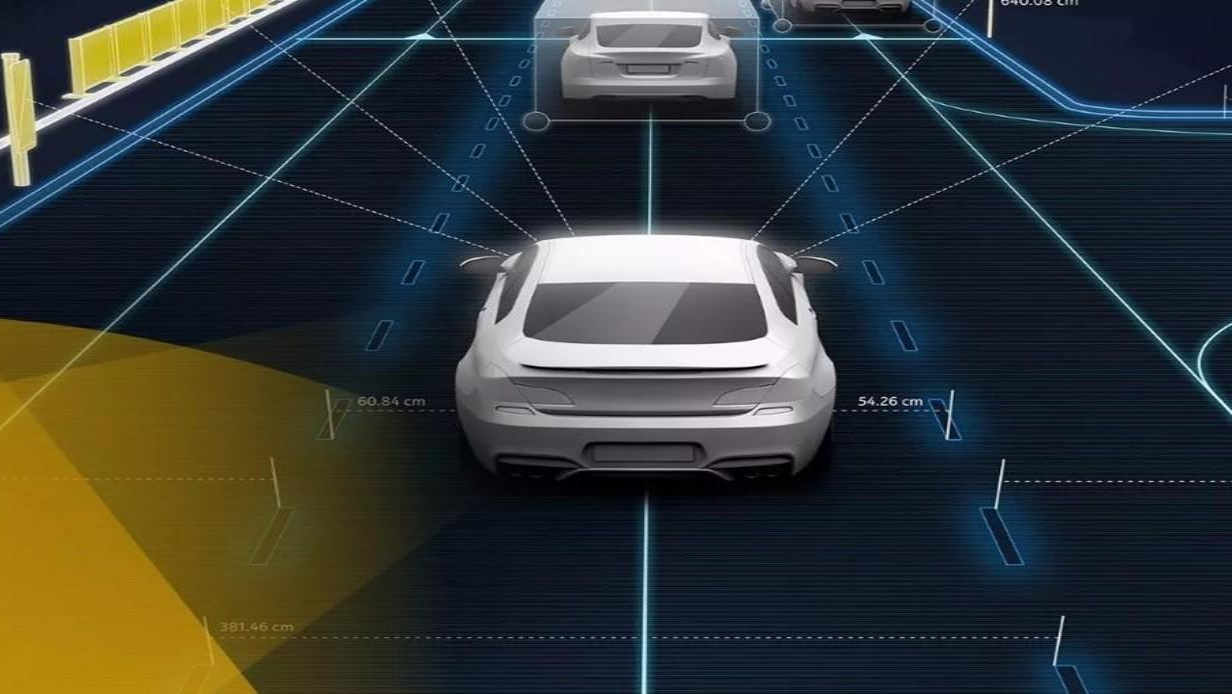
\includegraphics[width=0.7\textwidth]{autodrive.png}
	% footnotemark和footnotetext配合可以标注图片来源
	\caption{自动驾驶中的环境建模\protect\footnotemark[1]}
	\label{fig:introduction:autodrive}
	\addtocounter{figure}{-1}
	\renewcommand{\figurename}{Fig.}
	\caption{The environment reconstruction in automatic driving}
\end{figure}
\footnotetext[1]{图片来自于网络 http://auto.eastday.com/a/180720170248887.html}

\subsubsection{minipage}
minipage示例如图\ref{fig:line_optim:input}所示。

\begin{figure}[htb]
	\centering
	\begin{minipage}[t]{0.45\textwidth}
		\centering
		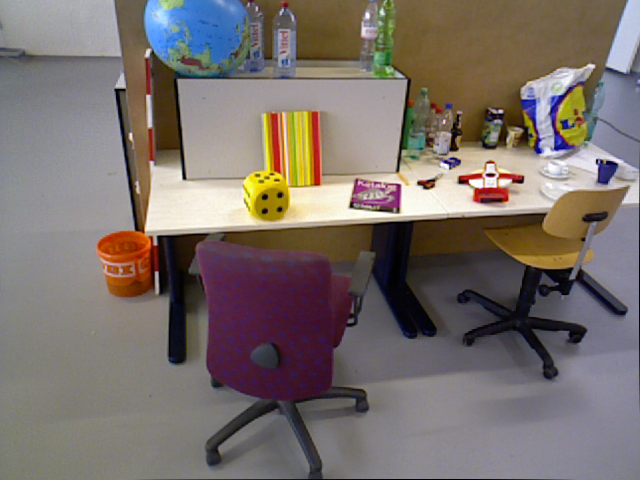
\includegraphics[width=0.8\textwidth]{tum-fr3-office-input1.png}
		\subcaption{场景输入图1}
		\label{fig:line_optim:input1}
	\end{minipage}
	\vspace{0.1in} %纵向间距,单位in或cm或pt等
	\begin{minipage}[t]{0.45\textwidth}
		\centering
		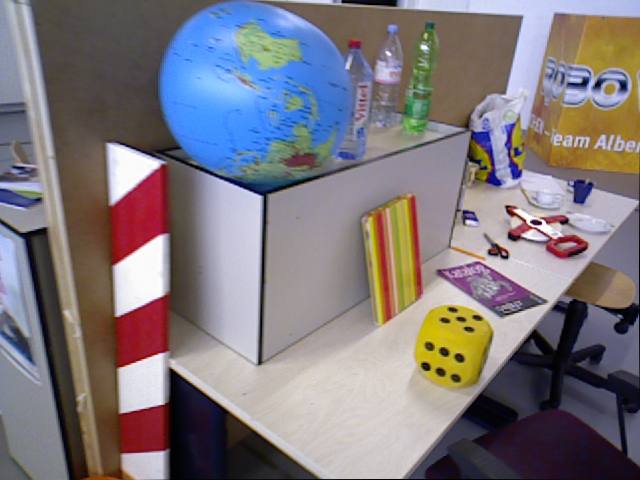
\includegraphics[width=0.8\textwidth]{tum-fr3-office-input2.png}
		\subcaption{场景输入图2}
		\label{fig:line_optim:input2}
	\end{minipage}
	\vspace{0.1in}
	\caption{TUM数据集{\itshape fr3\_long\_office}序列输入图}
	\label{fig:line_optim:input}
	\addtocounter{figure}{-1} %必须计数减一,否则上下中英标题的序号会递增
	\renewcommand{\figurename}{Fig.}
	\caption{The input images of {\itshape fr3\_long\_office} sequence in TUM dataset}
\end{figure}

\subsubsection{subfugure}
subfigure示例如图\ref{fig:line_optim:map}所示。

\begin{figure}[htb]
	\centering
	% subfigure[场景输入图像]{}
    \begin{subfigure}[b]{0.8\textwidth}
		\centering
		% 并排两个图像,也可以使用“\\”换行,改为纵向排列
        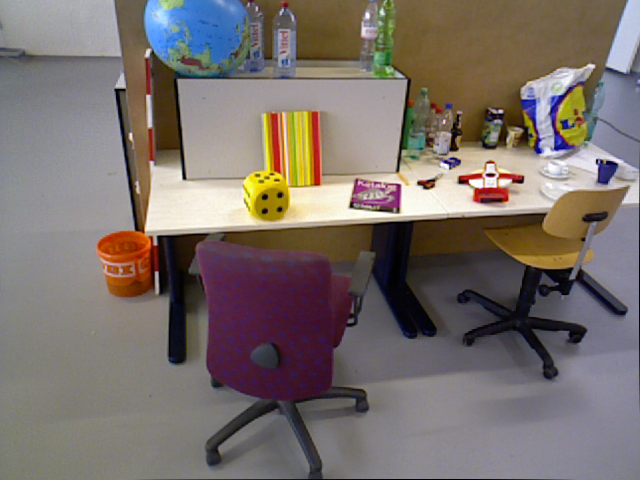
\includegraphics[width=0.45\textwidth]{tum-fr3-office-input1.png} %\\
        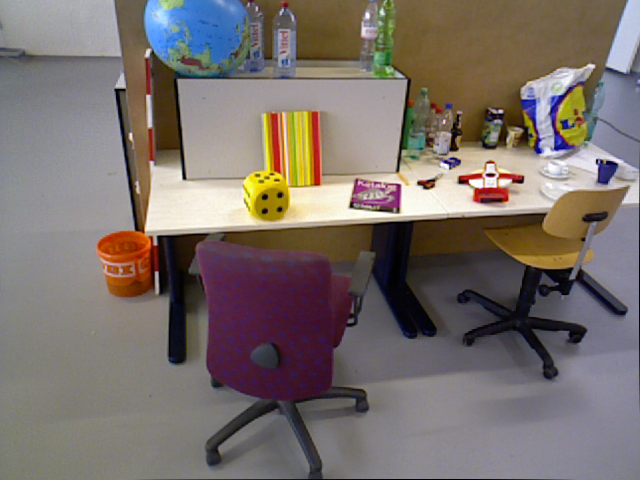
\includegraphics[width=0.45\textwidth]{tum-fr3-office-input1.png}
        \caption{场景输入图像}
    \end{subfigure}
    \vspace{0.3cm}
    \begin{subfigure}[b]{0.45\textwidth}
        \centering
        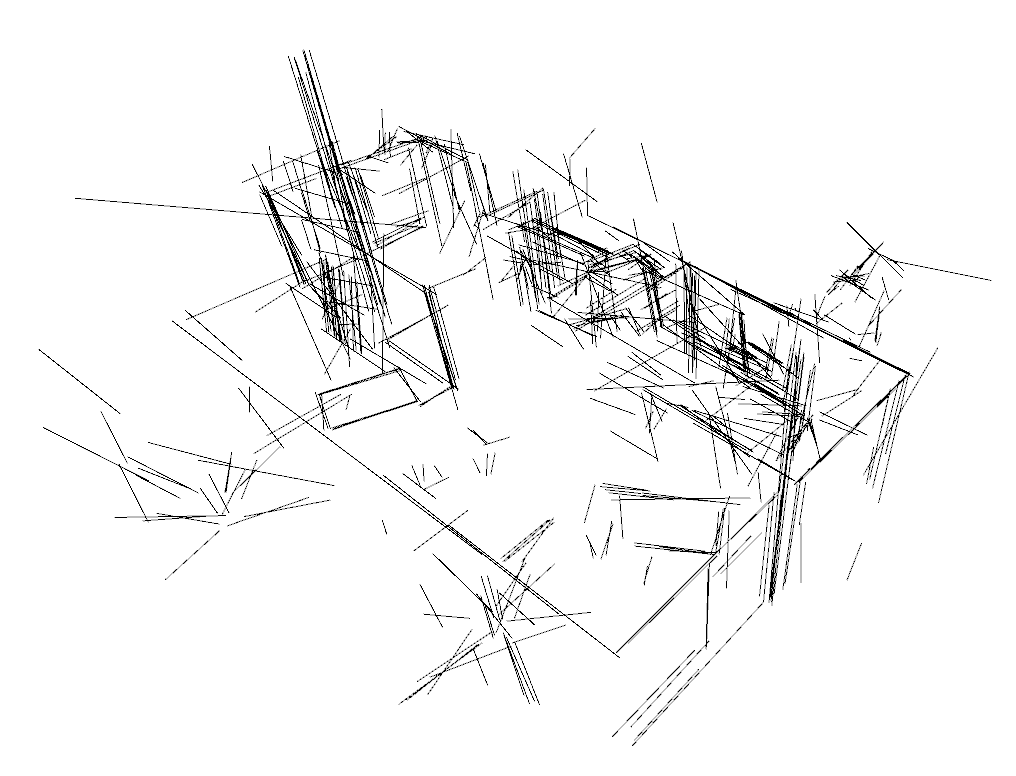
\includegraphics[width=0.9\textwidth]{line-map-TUM-fr3-office-lf.png}
        \caption{LF-SLAM算法的重建结果}
    \end{subfigure}
    \vspace{0.2cm}
    \begin{subfigure}[b]{0.45\textwidth}
        \centering
        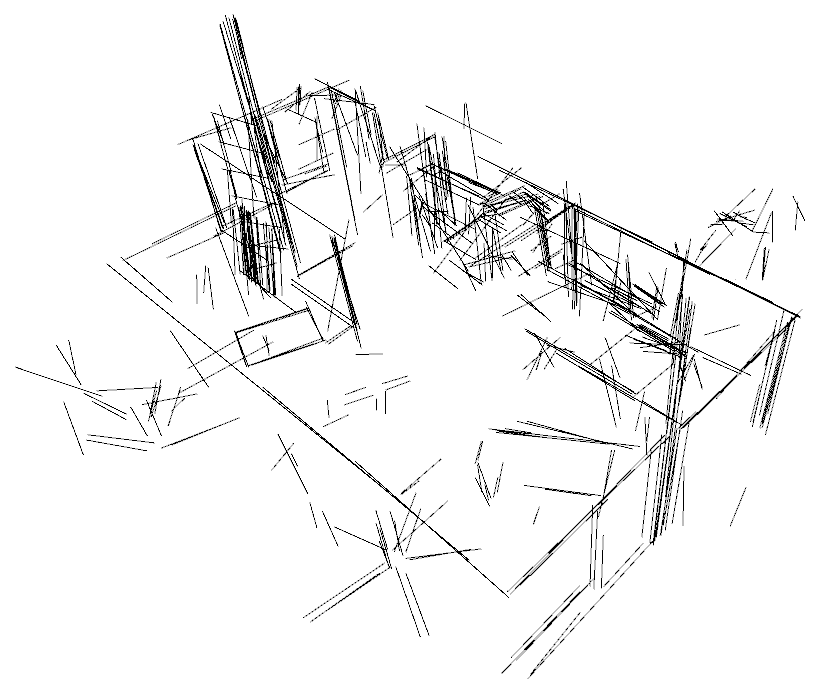
\includegraphics[width=0.9\textwidth]{line-map-TUM-fr3-office-ours.png}
        \caption{本章算法的重建结果}
    \end{subfigure}
    \vspace{0.2cm}
	\caption{在TUM {\itshape fr3\_long\_office}序列上的重建结果}
    \label{fig:line_optim:map}
    \addtocounter{figure}{-1}
    \renewcommand{\figurename}{Fig.}
    \caption{The results of mapping on {\itshape fr3\_long\_office} sequence in TUM}
\end{figure}

\subsection{表格}

tzz表格如111111111111111下所示:

\begin{table}[htb]
	\vspace{-0.5cm}                   %中文标题与上文距离
    \centering
	\small
	\setlength{\abovecaptionskip}{-0.3cm}
	\setlength{\belowcaptionskip}{0.3cm} 
	\caption*{test的表格}
	\caption*{test's table} 
	\begin{center}
		% c 居中,l 左对齐,r 右对齐,t 指定列宽,顶部对齐,b 底部对齐,p 指定列宽,顶部对齐, m 指定列宽,居中对齐
		% | 表格竖线
        \begin{tabular*}{\hsize}{@{}@{\extracolsep{\fill}}ccc@{}}
		\toprule[0.75pt]
		数据集	&ORB-SLAM	&PL-SLA	\\
        \midrule[0.5pt]
        TUMaaaaaaaaa			&20.6aaaaaaaaa 		&45.9cccccccc	\\
        7-Scenesaaaaaaa	&20.0bbbbbbbbbbb		&45.4ccccccccc	\\
		\bottomrule[0.75pt]
        \end{tabular*}
	\end{center}
	\vspace{-0.7cm}    %表格与下文距离
\end{table}
文字文字文字文字文字文字文字文字文字文字文字文字文字文字文字文字文字文字文字文字文字文字文字文字文字文字
文字文字文字文字文字文字文字文字文字。
\begin{table}[htb]
	\label{tab:parametervalues}
	\caption*{参数数值表}
	\caption*{Parameter values Table}
	\begin{tabular*}{\hsize}{@{}@{\extracolsep{\fill}}ccc@{}}
	\toprule[0.75pt]
	$p_{t}$  &21  &22\\
	\midrule[0.5pt]
	$c_{t}$aaaaaaaaaaaa  &EFI\_SIMPLE\_TEXT\_INPUT\_PROTOCOL*   &\makecell[c]{13caaaaaa\\aaaaaaaa\\cccc}\\
	$h_{t}$aaaaaaaaaaaa  &10bbbbbbbbb  &5ccccccccc\\
	\bottomrule[0.75pt]
	\end{tabular*}
	\vspace{-0.3cm}    %表格与下文距离
\end{table}
文字文字文字文字文字文字文字文字文字文字文字文字文字文字文字文字文字文字文字文字文字文字文字文字文字文字
文字文字文字文字文字文字文字文字文字。文字文字文字文字文字文字文字文字文字文字文字文字文字文字文字文字文字文字文字文字文字文字文字文字文字文字
文字文字文字文字文字文字文字文字文字。文字文字文字文字文字文字文字文字文字文字文字文字文字文字文字文字文字文字文字文字文字文字文字文字文字文字
文字文字文字文字文字文字文字文字文字。文字文字文字文字文字文字文字文字文字文字文字文字文字文字文字文字文字文字文字文字文字文字文字文字文字文字
文字文字文字文字文字文字文字文字文字。文字文字文字文字文字文字文字文字文字文字文字文字文字文字文字文字文字文字文字文字文字文字文字文字文字文字
文字文字文字文字文字文字文字文字文字。文字文字文字文字文字文字文字文字文字文字文字文字文字文字文字文字文字文字文字文字文字文字文字文字文字文字
文字文字文字文字文字文字文字文字文字。
\subsection{列表}

\subsubsection{enumerate}
enumerate列表带编号,默认样式1.

\begin{enumerate}[(1)]
	\item 分析现有SLAM框架的优势和不足,提出一种多视角互补的SLAM框架,该框架对现有框架做了改进,相比于现有框架,利用了观测数据的帧间约束信息,在位姿精度和重建效果方面提供了更大的提升空间。
	\item 在多视角互补框架下,结合多视角观测信息,提出一种可信度量方式,尽可能地降低不可靠特征对位姿优化带来的干扰,提升相机定位精度。
	\item 在多视角互补框架下,利用前后帧的观测信息,求解相机位姿和三维特征信息,同时也对局部帧的二维线条进行反向优化,提升线条完整度和端点的准确度,从而提升重建质量。
	\item 在多视角互补框架下,融合点线面特征,构建复合特征,在复合特征结构下,优化求解相机位姿和三维地图,提升优化速度和位姿精度,提高地图重建质量。 
\end{enumerate}

\subsubsection{itemize}
itemize列表

\begin{itemize}
\item 第1章\quad 绪论

\item 第2章\quad 相关知识及数据集

\item 第3章\quad 基于多视角互补的SLAM框架

\item 第4章\quad 基于多视角互补的捆绑优化算法

\item 第5章\quad 基于多视角互补的线条优化算法

\item 第6章\quad 基于多视角互补的复合特征优化算法

\item 结论

\end{itemize}

\bjutclearpage